\documentclass[../../main.tex]{subfiles}
\begin{document}

{\bf [解]}
正の整数$m,n$が
\begin{align}
 1\le m,n\le2N \label{eq:1}
\end{align}
を満たすとする．
$f(x)=x^2-nx+m$とおく．$f(x)=0$が$N$以上の実数解を持つ条件を考える．
$f$の軸は$x=\dfrac{n}{2}$であり，\cref{eq:1}よりこれは$\dfrac{n}{2}\le N$を満たす．
放物線$y=f(x)$は下に凸で軸が$N$以下にあるから，「$N$以上の実数解を持つ」ことと「$f(N)\le 0$」は同値である．
よって条件は
\begin{align}
f(N)=N^2-nN+m\le0\quad\therefore\ m\le Nn-N^2\equiv g(n) \label{eq:2}
\end{align}
である．\cref{eq:1,eq:2}を満たす$(m,n)$の組を数えれば良い．
これを$nm$平面上に図示すると，直線$m=Nn-N^2$は$n=N$で$m=0$，$n=N+2$で$m=2N$を通るので以下のようになる．境界は$m=0$のみ含まない．$N=1$と$N \ge 2$の場合でそれぞれ場合分けして考える．

\begin{figure}[htb]
\centering
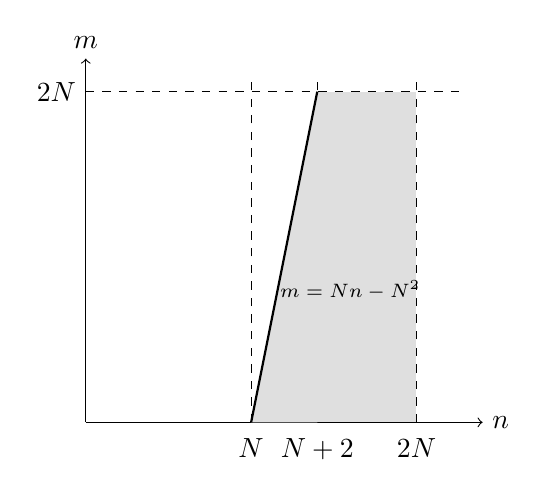
\begin{tikzpicture}[scale=0.42]
  % N=5として図示
  \def\N{5}
  \draw[->] (0,0) -- (12,0) node[right]{$n$};
  \draw[->] (0,0) -- (0,11) node[above]{$m$};
  \draw[dashed] (\N,0) -- (\N,10.5);
  \draw[dashed] ({\N+2},0) -- ({\N+2},10.5);
  \draw[dashed] (2*\N,0) -- (2*\N,10.5);
  \draw[dashed] (0,2*\N) -- (11.5,2*\N);
  \node[below] at (\N,-0.2) {$N$};
  \node[below] at ({\N+2},-0.2) {$N+2$};
  \node[below] at (2*\N,-0.2) {$2N$};
  \node[left] at (0,2*\N) {$2N$};
  % n=N..N+2: 境界線 m=Nn-N^2 の下側 (0からNまで上昇)
  \fill[gray!25] plot[domain=\N:{\N+2},samples=2] (\x,{\N*\x-\N*\N}) -- ({\N+2},0) -- (\N,0) -- cycle;
  % n=N+2..2N: 上限m=2Nが効き、m=1..2Nの全域
  \fill[gray!25] ({\N+2},0) rectangle (2*\N,2*\N);
  \draw[thick,domain=\N:{\N+2},samples=2] plot (\x,{\N*\x-\N*\N});
  \node at (8,4) {\scriptsize$m=Nn-N^2$};
\end{tikzpicture}
\caption{条件①，②をみたす領域（斜線部，$N\ge3$の場合の概形）}
\end{figure}

\begin{figure}[htb]
\begin{center}
\begin{tikzpicture}[scale=1.15, >=stealth]

  % --- 1. 設定 (N = 3, 2N = 6 の具体例で格子点と領域をプロット) ---
  \def\N{3}
  \pgfmathsetmacro{\twoN}{2*\N} % 6

  % --- 2. 条件を満たす領域のハッチング (1 <= m <= min(Nn - N^2, 2N)) ---
  % n = N+1 (=4): 1 <= m <= N (=3)
  % n = N+2..2N (=5..6): 1 <= m <= 2N (=6)
  \fill[pattern=north east lines, pattern color=blue!60] 
    (\N, 0) -- ({\N+2}, \twoN) -- (\twoN, \twoN) -- (\twoN, 0) -- (\N, 0) -- cycle;

  % --- 3. 座標軸 ---
  \draw[->, thick] (-0.5, 0) -- ({\twoN + 1.2}, 0) node[right] {$n$};
  \draw[->, thick] (0, -0.5) -- (0, {\twoN + 1.2}) node[above] {$m$};
  \node[below left, font=\small] at (0,0) {$O$};

  % --- 4. 全体枠 1 <= n, m <= 2N のガイド線 ---
  \draw[dashed, gray!60] (1, 1) rectangle (\twoN, \twoN);
  \draw[dashed, gray!60] (\twoN, 0) -- (\twoN, 1);
  \draw[dashed, gray!60] (0, \twoN) -- (1, \twoN);
  \draw[dashed, gray!60] (0, 1) -- (1, 1);
  \draw[dashed, gray!60] (1, 0) -- (1, 1);

  % --- 5. 境界線 m = Nn - N^2 の描画 ---
  % (N, 0) から (N+2, 2N) を結ぶ直線
  \draw[ultra thick, blue!80!black] (\N, 0) -- ({\N+2}, \twoN)
    node[midway, above left, font=\small, sloped] {$m = Nn - N^2$};

  % 上限 m = 2N の頭打ち境界
  \draw[ultra thick, blue!80!black] ({\N+2}, \twoN) -- (\twoN, \twoN);

  % --- 6. 全格子点のプロット (1 <= n, m <= 2N) ---
  \foreach \x in {1,...,\twoN} {
    \foreach \y in {1,...,\twoN} {
      % 条件判定: y <= N*x - N*N
      \pgfmathsetmacro{\mBound}{\N*\x - \N*\N}
      \ifnum \y > \mBound
        % 条件を満たさない点 (薄い灰色)
        \fill[gray!40] (\x, \y) circle (1.2pt);
      \else
        % 条件を満たす点 (赤色で強調)
        \fill[red!80!black] (\x, \y) circle (2.0pt);
      \fi
    }
  }

  % --- 7. 目盛りとラベル ---
  % 横軸目盛り
  \draw[dashed, gray] (\N, 0) -- (\N, -0.1);
  \node[below, font=\small] at (\N, 0) {$N$};
  
  \draw[dashed, gray] ({\N+1}, 0) -- ({\N+1}, \N);
  \node[below, font=\small] at ({\N+1}, 0) {$N+1$};
  
  \draw[dashed, gray] ({\N+2}, 0) -- ({\N+2}, \twoN);
  \node[below, font=\small] at ({\N+2}, 0) {$N+2$};

  \node[below, font=\small] at (\twoN, 0) {$2N$};

  % 縦軸目盛り
  \draw[dashed, gray] (0, \N) node[left, font=\small] {$N$} -- ({\N+1}, \N);
  \draw[dashed, gray] (0, \twoN) node[left, font=\small] {$2N$} -- ({\N+2}, \twoN);
  \node[left, font=\small] at (0, 1) {$1$};

  % --- 8. 各列の個数の注記 ---
  % n = N+1 の列: N 個
  \draw[<->, thin, red!80!black] ({\N+1 + 0.25}, 1) -- ({\N+1 + 0.25}, \N)
    node[midway, right, font=\scriptsize] {$N$ 個};

  % n = 2N の列: 2N 個
  \draw[<->, thin, red!80!black] ({\twoN + 0.25}, 1) -- ({\twoN + 0.25}, \twoN)
    node[midway, right, font=\scriptsize] {$2N$ 個};

\end{tikzpicture}
\end{center}
\caption{$N \ge 2$の時条件を満たす格子点}
\end{figure}

\begin{figure}[htb]
\begin{center}
\begin{tikzpicture}[scale=1.8, >=stealth]

  % --- 1. 座標軸 ---
  \draw[->, thick] (-0.3, 0) -- (3.2, 0) node[right] {$n$};
  \draw[->, thick] (0, -0.3) -- (0, 3.2) node[above] {$m$};
  \node[below left, font=\small] at (0,0) {$O$};

  % --- 2. 全体枠 1 <= n, m <= 2 (2N=2) のガイド線 ---
  \draw[dashed, gray!60] (1, 1) rectangle (2, 2);
  \draw[dashed, gray!60] (2, 0) -- (2, 1);
  \draw[dashed, gray!60] (0, 2) -- (1, 2);
  \draw[dashed, gray!60] (0, 1) -- (1, 1);
  \draw[dashed, gray!60] (1, 0) -- (1, 1);

  % --- 3. 境界線 m = n - 1 (N=1) ---
  % (1,0) から (3,2) への直線
  \draw[ultra thick, blue!80!black, domain=0.8:2.8] plot (\x, {\x - 1})
    node[above left, font=\small] {$m = n - 1$};

  % --- 4. 格子点のプロット (1 <= n, m <= 2 の4点) ---
  % 条件を満たさない点 (灰色)
  \fill[gray!40] (1, 1) circle (1.8pt);
  \fill[gray!40] (1, 2) circle (1.8pt);
  \fill[gray!40] (2, 2) circle (1.8pt);

  % 唯一条件を満たす点 (2, 1) (赤色で強調)
  \fill[red!80!black] (2, 1) circle (2.4pt);
  \draw[red!80!black, thick] (2, 1) circle (5.0pt);
  \node[red!80!black, font=\small, below right] at (2.05, 0.95) {$(2,1)$ (1個)};

  % --- 5. 目盛りとラベル ---
  % 横軸
  \node[below, font=\small] at (1, 0) {$1\ (N)$};
  \node[below, font=\small] at (2, 0) {$2\ (2N)$};

  % 縦軸
  \node[left, font=\small] at (0, 1) {$1$};
  \node[left, font=\small] at (0, 2) {$2\ (2N)$};

\end{tikzpicture}
\end{center}
\caption{$N=1$ のときの条件を満たす格子点（$(n,m)=(2,1)$ の 1 個のみ）}
\end{figure}

\subparagraph{$N \ge 2$の時}

図から条件を満たすのは$n=N+1,\dots,2N$の時のみである．
それぞれについて対応する$m$の数を数えると，

\begin{itemize}
\item $n=N+1$：$g(N+1)=N$より，$m=1,\dots,N$の$N$通りが対応する．
\item $n=N+2,\dots,2N$：$g(n)\ge2N$となり$m$の上限$2N$が効くので，各列$m=1,\dots,2N$の$2N$通りが対応する．
\end{itemize}

よって，もとめる組の総数を$F(N)$とすると
\begin{align}
F(N)=N+(N-1)\cdot2N=N+2N^2-2N=N(2N-1) \label{eq:3}
\end{align}
である．

\subparagraph{$N=1$の時}

この時は図より$(n,m)=(2,1)$のみが対応して
\begin{align}
 F(1) = 1
\end{align}
であり，\cref{eq:3}の表現で良い．
\casesend

以上より，すべての正の整数$N$に対して，求める組$(m,n)$の個数は
\begin{align}
N(2N-1)
\end{align}
である．


\newpage

\end{document}
